
\chapter{Algorithm and Analysis}
\label{ch:analysis}



In this chapter, we present our main randomized median-finding algorithm in full detail and analyze its performance. We first give a high-level description and provide the pseudocode in Algorithm~\ref{alg:randmedian}. We then prove two central theorems: one that establishes the algorithm’s probability of success (i.e.\ returning the correct median) and another that bounds its running time by \Oh*{n}. Throughout this chapter, we use the notation introduced in Chapter~\ref{ch:notation}.
\section*{Algorithm Description}

The guiding idea behind the algorithm is to select a “small” random sample from the input array, sort this sample, and use carefully chosen elements from this sample as \emph{pivots} to bracket the true median. Specifically:
\begin{itemize}
    \item We draw \( m = \lceil n^{3/4} \rceil \) elements uniformly at random from the input array \( a[1 \dots n] \) and sort these sampled elements into an array \( b[1 \dots m] \).
    \item We then pick two elements from \( b \), denoted \( p_\ell \) and \( p_r \), near the middle of \( b \) but offset by \(\pm \sqrt{n}\). Intuitively, these two pivots should “sandwich” the true median of the entire array with high probability.
    \item We gather all elements of the original array \( a \) that lie between these two pivots (inclusive) into a temporary array \(T\). We verify that the median must lie in this sub-array, and that \(T\) is not excessively large.
    \item If those checks are satisfied, we sort \(T\) and extract the median; otherwise, the algorithm reports a \emph{failure}.
\end{itemize}
\begin{algorithm}
    \caption{RandMedian: Randomized Median Algorithm}
    \label{alg:randmedian}
    \begin{algorithmic}[1]
    \Require Unsorted array \( a[1 \dots n] \) of size \( n \).
    \Ensure Median of \( a \) or \emph{failure}.
    
    \State \textbf{Initialize} an empty array \(b\).
    \State \textbf{For each} element \(x \in a[1 \dots n]\):
    \Statex \quad \textbf{Include} \(x\) in \(b\) \textbf{with probability} \(n^{-1/4}\), independently of other elements.
    \State \( m \gets |b| \) 
        \Comment{(Random) size of the sample; note that \(\E{m} = n^{3/4}\).}

    \If{\( m > n^{3/4} + \sqrt{n} \)}
        \State \Return \emph{failure}
    \EndIf

    \State \textbf{Sort} \( b \) in \(\Oh*{m \log m}\) time
    
    \State \textbf{Compute pivots}:
    \[
      p_\ell \gets b\Bigl[\Bigl\lfloor \tfrac{m}{2} - \sqrt{n} \Bigr\rfloor\Bigr], 
      \quad
      p_r \gets b\Bigl[\Bigl\lceil \tfrac{m}{2} + \sqrt{n} \Bigr\rceil\Bigr]
    \]
    
    \State Define the subset \( T \gets \{\, x \in a : p_\ell \le x \le p_r \}\)
    
    \State Compute:
    \begin{align*}
        s &\gets \#\{\, x \in a : x < p_\ell \},\\
        t &\gets \#\{\, x \in a : p_\ell \le x \le p_r \}.
    \end{align*}
    
    \If{\( s < \lceil n/2 \rceil \)\textbf{ and }\( s + t \ge \lceil n/2 \rceil \)\textbf{ and }\( t < 4n^{3/4}\)} \label{alg:randmedian:check}
        \State \textbf{Sort} \( T \) in \(\Oh*{|T|\log |T|}\) time
        \State \(\text{Median of } a \;\gets\; T[\lceil n/2 \rceil - s]\)
        \State \Return \(\text{Median of } a\)
    \Else
        \State \Return \emph{failure}
    \EndIf
    \end{algorithmic}
    \end{algorithm}
    

The rest of this chapter gives a proof of two properties of this algorithm:
\begin{enumerate}
    \item With high probability, Algorithm~\ref{alg:randmedian} does not fail and returns the correct median.
    \item Conditioned on success, the overall running time is \Oh*{n}.
\end{enumerate}

\section*{Probability of Success}





\begin{figure}[htbp]
    \centering
    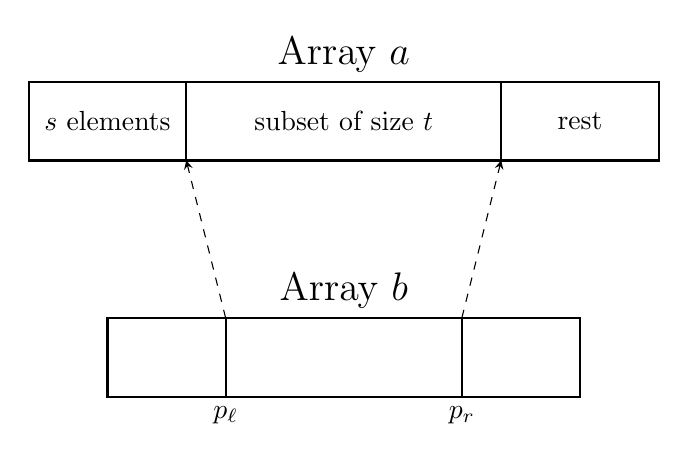
\begin{tikzpicture}[>=stealth, scale=1]
  
        % 1) Draw a big rectangle for array 'a'
        \draw[thick] (0,0) rectangle (8,1);
        \node[above] at (4,1) {\Large Array $a$};
  
        % 2) Draw a smaller rectangle for array 'b' (below 'a')
        \draw[thick] (1,-2) rectangle (7,-3);
        \node[above] at (4,-2) {\Large Array $b$};
  
        % 3) Mark p_l and p_r in 'b'
        \draw[thick] (2.5,-2) -- (2.5,-3); 
        \draw[thick] (5.5,-2) -- (5.5,-3); 
        \node[below] at (2.5,-3) {$p_\ell$};
        \node[below] at (5.5,-3) {$p_r$};
  
        % 4) Arrows from pivots in 'b' up to partitions in 'a'
        \draw[dashed,->] (2.5,-2) -- (2,0);
        \draw[dashed,->] (5.5,-2) -- (6,0);
  
        % Vertical lines in 'a' to show partition
        \draw[thick] (2,0) -- (2,1); 
        \draw[thick] (6,0) -- (6,1); 
  
        % 5) Label the segments in 'a'
        \node at (1,0.5) {$s$ elements};
        \node at (4,0.5) {subset of size $t$};
        \node at (7,0.5) {rest};
  
    \end{tikzpicture}
    \caption{Illustration of the arrays and the pivots, showing array $a$, sampled array $b$, and the pivots $p_\ell, p_r$. Note that this visualization shows the sorted version of the arrays.}
    \label{fig:randmedian}
  \end{figure}
  






We begin by showing that, except with small probability, the two pivots \(p_\ell\) and \(p_r\) are chosen so that the sub-array \(T\) contains the true median of \(a\) and is not excessively large. Formally, we have:

\begin{theorem}[Correctness with High Probability]
    \label{thm:correctness}
    The probability that~\Cref{alg:randmedian} returns the correct median is at least \(1 - \Oh*{n^{-1/4}}\). In other words, the algorithm succeeds \emph{with high probability}.
    \end{theorem}
    
    \begin{proof}
    For simplicity, we assume throughout this proof that \(n\) is even and that \(n^{3/4}\) is an integer; this avoids cumbersome floor and ceiling functions. The general case follows by analogous, but slightly more tedious, arguments.
    
    Recall that \(a[\,1\dots n\,]\) is our input array of \(n\) distinct elements. Let \(b[\,1\dots m\,]\) be the sample of size \(m\) drawn by sampling each element with probability $n^{-1/4}$ from \(a\). The setup is also visualized in~\Cref{fig:randmedian}. We then sort \(b\), pick the pivots\footnote{Technically, if $m$ is too small, the following lines are undefined (out of bounds). But this is avoided whp, as for the other events later in the proof.}
    \[
    p_\ell \;=\; b\Bigl[\,\tfrac{m}{2} - \sqrt{n}\Bigr],
    \quad
    p_r \;=\; b\Bigl[\,\tfrac{m}{2} + \sqrt{n}\Bigr],
    \]
    and collect into \(T\) all elements \(x \in a\) with \(p_\ell \le x \le p_r\). Let
    \[
    s \;=\; \#\SetBuilder{x\in a}{x < p_\ell}
    \quad\text{and}\quad
    t \;=\; \#\SetBuilder{x\in a}{p_\ell \le x \le p_r}.
    \]
    \paragraph{Key sets and random variables.}
For any integer \(k \in \{0,\dots,n\}\), define
\[
   S_k \;=\; \{\text{the }k \text{ smallest elements of } a\}.
\]
We then define the random variable
\[
   X_k \;=\; \#\{\, x \in b : x \in S_k \}.
\]
Since each element of \(a\) is independently included in \(b\) with probability \(n^{-1/4}\),
the number of elements of \(S_k\) that appear in \(b\) follows
\[
   X_k \;\sim\; \mathrm{Bin}\bigl(k,\;n^{-1/4}\bigr).
\]
Hence,
\[
   \E{X_k} \;=\; k\,n^{-1/4},
   \quad
   \Var{X_k} \;=\; k\,n^{-1/4}\bigl(1 - n^{-1/4}\bigr)
   \;\le\;
   k\,n^{-1/4}.
\]

    
    \paragraph{Application of Chebyshev’s Inequality.}
    Since \(X_k \sim \mathrm{Bin}(k,\,n^{-1/4})\) with 
\(\Var{X_k} \le k\,n^{-1/4},\)
Chebyshev’s inequality gives
\begin{equation}
    \Prob{\bigl|X_k - k\,n^{-1/4}\bigr|\;\ge\;\sqrt{n}}
    \;\;\le\;\;
    \frac{\Var{X_k}}{\,n\,}
    \;\;\le\;\;
    \frac{k\,n^{-1/4}}{n}
    \;=\;
    \frac{k}{n^{5/4}}. \label{eq:fail}   
\end{equation}
    \paragraph{Defining the “bad” events.}
    We show that the only way the algorithm can fail (i.e.\ not return the correct median) is if one of the following four events occurs. Denote
    \begin{align*}
    A \;&:=\; \{\, s \;\ge\; n/2 \}\,,
    \\
    B \;&:=\; \{\, s + t < n/2 \}\,,
    \\
    C \;&:=\; \{\, s < \tfrac{n}{2} - 2\,n^{3/4} \}\,,
    \\
    D \;&:=\; \{\, s + t \;\ge\; \tfrac{n}{2} + 2\,n^{3/4} \}\,.
    \\
    E \;&:=\; \{\, m > n^{3/4} + \sqrt{n} \}\,.
    \end{align*}
    Notice that $E$ not occuring means that the first ``return failure'' line is not executed. If none of these events happens, then we must have
    \[
    s < \tfrac{n}{2}, 
    \quad
    s + t \;\ge\; \tfrac{n}{2},
    \quad
    s \;\ge\; \tfrac{n}{2} - 2\,n^{3/4},
    \quad
    \text{and}
    \quad
    s + t < \tfrac{n}{2} + 2\,n^{3/4}.
    \]
    One can check that these conditions imply exactly
    \[
    \bigl(s < \tfrac{n}{2}\bigr)
    \quad\text{and}\quad
    \bigl(s + t \ge \tfrac{n}{2}\bigr)
    \quad\text{and}\quad
    t < 4\,n^{3/4},
    \]
    so the algorithm’s final check (line~\ref{alg:randmedian:check} of the pseudocode) succeeds. In that case, our pivot-based bracket \([\,p_\ell,\,p_r\,]\) indeed contains the median, and the algorithm returns the correct value.
    
    \paragraph{Probability of each bad event.}
    We next prove that \(\Prob{A},\Prob{B},\Prob{C},\Prob{D},\Prob{E}\) are each at most \(n^{-1/4}\). Observe:
    \begin{itemize}
    \item Event \(A\) means \(s \ge n/2\). Hence among the \(n/2\) smallest elements of \(a\) (i.e.\ the set \(S_{n/2}\)), at most \(\tfrac12\,n^{3/4} - \sqrt{n}\) of them are drawn into \(b\). In other words,
    \[
    X_{\,n/2} \;\;\le\;\; \tfrac12\,n^{3/4} \;-\; \sqrt{n}.
    \]
    But from \(\E{X_{\,n/2}} = (n/2)\,n^{-1/4} = \tfrac12\,n^{3/4}\) and \eqref{eq:fail}, we get 
    \(\Prob{X_{\,n/2} \le \tfrac12\,n^{3/4} - \sqrt{n}} \le n^{-1/4}\). Thus \(\Prob{A} \le n^{-1/4}\).
    
    \item Event \(B\) means \(s+t < n/2\). Equivalently, the set \(S_{n/2}\) has more than \(\tfrac12\,n^{3/4} + \sqrt{n}\) elements contained in \(b\). Hence
    \[
    X_{\,n/2} \;\;\ge\;\; \tfrac12\,n^{3/4} \;+\; \sqrt{n}.
    \]
    Again, from \(\E{X_{\,n/2}} = \tfrac12\,n^{3/4}\) and \eqref{eq:fail}, we get 
    \(\Prob{X_{\,n/2} \ge \tfrac12\,n^{3/4} + \sqrt{n}} \le n^{-1/4}\). So \(\Prob{B}\le n^{-1/4}\).
    
    \item Event \(C\) means \(s < n/2 - 2\,n^{3/4}\). In this case, the set \(S_{\,n/2 - 2\,n^{3/4}}\) must have at least \(\tfrac12\,n^{3/4} - \sqrt{n}\) of its elements in \(b\). Formally,
    \[
    X_{\,n/2 - 2\,n^{3/4}} \;\;\ge\;\; \tfrac12\,n^{3/4}-\sqrt{n}.
    \]
    Using \(\E{X_{\,n/2 - 2\,n^{3/4}}} = (n/2 - 2\,n^{3/4})\,n^{-1/4} = \frac{1}{2}n^{3/4} - 2\sqrt{n}\)  and \eqref{eq:fail} again shows 
    \(\Prob{C} \le n^{-1/4}\).
    
    \item Event \(D\) means \(s+t \ge n/2 + 2\,n^{3/4}\). Hence the set \(S_{\,n/2 + 2\,n^{3/4}}\) contains at most \(\tfrac12\,n^{3/4} + \sqrt{n}\) elements from \(b\). That is,
    \[
    X_{\,n/2 + 2\,n^{3/4}} 
    \;\;\le\;
    \tfrac12\,n^{3/4} \;+\; \sqrt{n}.
    \]
    A final application of \eqref{eq:fail} yields \(\Prob{D}\le n^{-1/4}\).

    \item A similar calculation involving $X_n$ shows that \(\Prob{E}\le n^{-1/4}\).    
\end{itemize}

    \paragraph{Conclusion.}
    By the union bound,
    \[
    \Prob{A \,\cup\, B \,\cup\, C \,\cup\, D \cup\, E}
    \;\le\;
    \Prob{A}+\Prob{B}+\Prob{C}+\Prob{D}+\Prob{E}
    \;\le\;
    5\,\times n^{-1/4}
    \]
    In other words, with probability at least \(1 - 5n^{-1/4}\), \emph{none} of these events occurs. When all five do not occur, the algorithm’s checks
    \[
    s < \lceil n/2\rceil,\quad
    s + t \ge \lceil n/2\rceil,\quad
    t < 4\,n^{3/4}
    \]
    are satisfied, so the algorithm terminates successfully with the correct median. Hence the overall success probability is at least \(1 - 5n^{-1/4}\), completing the proof.
    \end{proof}
    

\section*{Runtime Analysis}

Next, we establish that Algorithm~\ref{alg:randmedian} achieves linear time complexity \emph{with high probability}. Note that if the algorithm returns \emph{failure}, it may be retried or combined with a fallback procedure. Here, we focus on the typical execution that succeeds.

\begin{theorem}[Runtime]
\label{thm:runningtime}
Conditioned on the event that Algorithm~\ref{alg:randmedian} does not fail (an event which, by Theorem~\ref{thm:correctness}, holds with high probability), the total running time is \Oh*{n}.
\end{theorem}

\begin{proof}
We break the cost into four parts:
\begin{enumerate}
    \item \textbf{Sampling and Sorting \(b\).}
    We pick \(m \le n^{3/4} + \sqrt{n} \le 2 n^{3/4}\) elements randomly from \(a\) (conditioned on success). This is done in \Oh*{n} time. Sorting \(b\) of size \(m\) then takes
    \[
    \Oh*{m \Log*{m}} 
    =
    \Oh*{n^{3/4} \Log*{n^{3/4}}}.
    \]
    Since \(n^{3/4} \Log*{n^{3/4}}\) is asymptotically smaller than \(n\) for large \(n\), this component is \oh*{n}.

    \item \textbf{Computing Ranks and Sub-array \(T\).}
    We determine how many elements of \(a\) lie below \(p_\ell\), how many lie above \(p_r\), etc. This amounts to a single pass through \(a\), comparing each element of \(a\) to \(p_\ell\) and \(p_r\). Hence, it costs \Oh*{n} time.

    \item \textbf{Sorting \(T\).}
    By Algorithm~\ref{alg:randmedian}, we only proceed to sort \(T\) if \(t < 4n^{3/4}\). Thus,
    \[
    t \le 4n^{3/4}.
    \]
    Sorting \(T\) via a standard comparison-based algorithm costs
    \[
    \Oh*{|T|\Log*{|T}|}
    \le
    \Oh*{n^{3/4} \Log*{\bigl(n^{3/4}\bigr)}},
    \]
    which again is \oh*{n}.

    \item \textbf{Extracting the Median.}
    After sorting \(T\), we simply pick the element of \(T\) whose rank corresponds to \(\lceil n/2\rceil - s\). This is clearly an \Oh*{1} operation.
\end{enumerate}

Summing these components, the \emph{dominant term} is \Oh*{n} (from the pass to identify \(s\) and \(t\)). The sublinear sorting costs on \(b\) and on \(T\) both constitute \Oh*{n^{3/4}\Log*{n}}, which is strictly smaller than \(n\) for large \(n\). Consequently, the total running time is \Oh*{n}.
\end{proof}

In conclusion, the previous two theorems immediately prove~\Cref{theorem:mainTheorem}, our main result, which we restate here for convenience.
\mainTheoremCommand*

\section*{Discussion and Extensions}

Theorems~\ref{thm:correctness} and~\ref{thm:runningtime} jointly show that Algorithm~\ref{alg:randmedian} achieves \Oh*{n} time with high probability of success. In rare cases where the check fails, the algorithm returns \emph{failure} rather than risking an incorrect answer. One can either re-run the algorithm (the probability of repeated failures being very low) or combine it with a fallback deterministic linear-time median-finding routine such as the median-of-medians approach. The randomized algorithm typically attains lower hidden constants in practice than purely deterministic linear-time solutions, thereby offering an attractive balance of theoretical guarantees and real-world performance.

In the next chapter, we summarize our results and highlight possible directions for future work on randomized selection algorithms.
